\documentclass[a4paper,13pt,openany,sffamily]{memoir}
\usepackage[T1]{fontenc}
\usepackage[utf8]{inputenc}
\usepackage{graphicx}
\usepackage{hyperref}
\usepackage{listings}
\usepackage{amsmath}
\usepackage{pdfpages}
\usepackage{geometry}

\pagenumbering{arabic}
\renewcommand{\chaptername}{}
\newgeometry{top=20mm, bottom=20mm, right=25mm, left=25mm}
%\geometry{a4paper, margin=20mm}


\sffamily

\pretitle{\begin{center}\Large \bfseries Final Report \\*}
\title{\Huge\bfseries ES-ESP5200 Modern Embedded Systems programming Coursework 2020}
\posttitle{\par\vskip1em{\normalfont\Large \bfseries \textit { Design, development, testing and evaluation of Slot Machine} \par\vfill}\end{center}}
\author{\LARGE \bfseries Biplav Karna}
%\date{\vfill\begin{center}\large November 2020}
\predate{\vfill\begin{center}\large}


%\let\stdsection\section
%\renewcommand\section{\newpage\stdsection}

\begin{document}

\maketitle

\chapter {Introduction}
Slot machine is a game device easily available at every game parlor and casino. Figure \ref{Fig_Casino_Slot_Machine} shows a slot machine. It has 3 spinning wheels, lever to start the spin, place to insert coin, display to show progress. It has some lighting effects and sound effects. 

\begin{figure}[htbp]
\centering{
\includegraphics[width=0.6\linewidth,keepaspectratio]{slot-machine-2304135_640.png}
}
\caption{General Slot Machine, PHOTO SRC: pixabay.com}
\label{Fig_Casino_Slot_Machine}
\end{figure}


This can be mimicked with avr 2560 with LCD screen, buttons, leds and speaker/buzzer.


\chapter {Design}
Slot machine is implemented using below components

\begin{itemize}
\item MEGA 2560 board
\item 16 * 2 LCD 
\item 10 LEDs
\item 4 * 4 Keypad (using only 2 button)
\item supporting connections and components 
\end{itemize}

The circuit diagram of the implementation is shown in the figure \ref{Fig_Circuit_Diagram}. PA0-PA7 are used for data bus, and PG0-PG2 are used for control bus for LCD interfacing. PB0-PB7 are used for LEDs. PD0-PD1 are connected to two buttons for spin and bet functions. PD0-PD1 are used as external interrupts. 

\begin{figure}[h]
\centering{
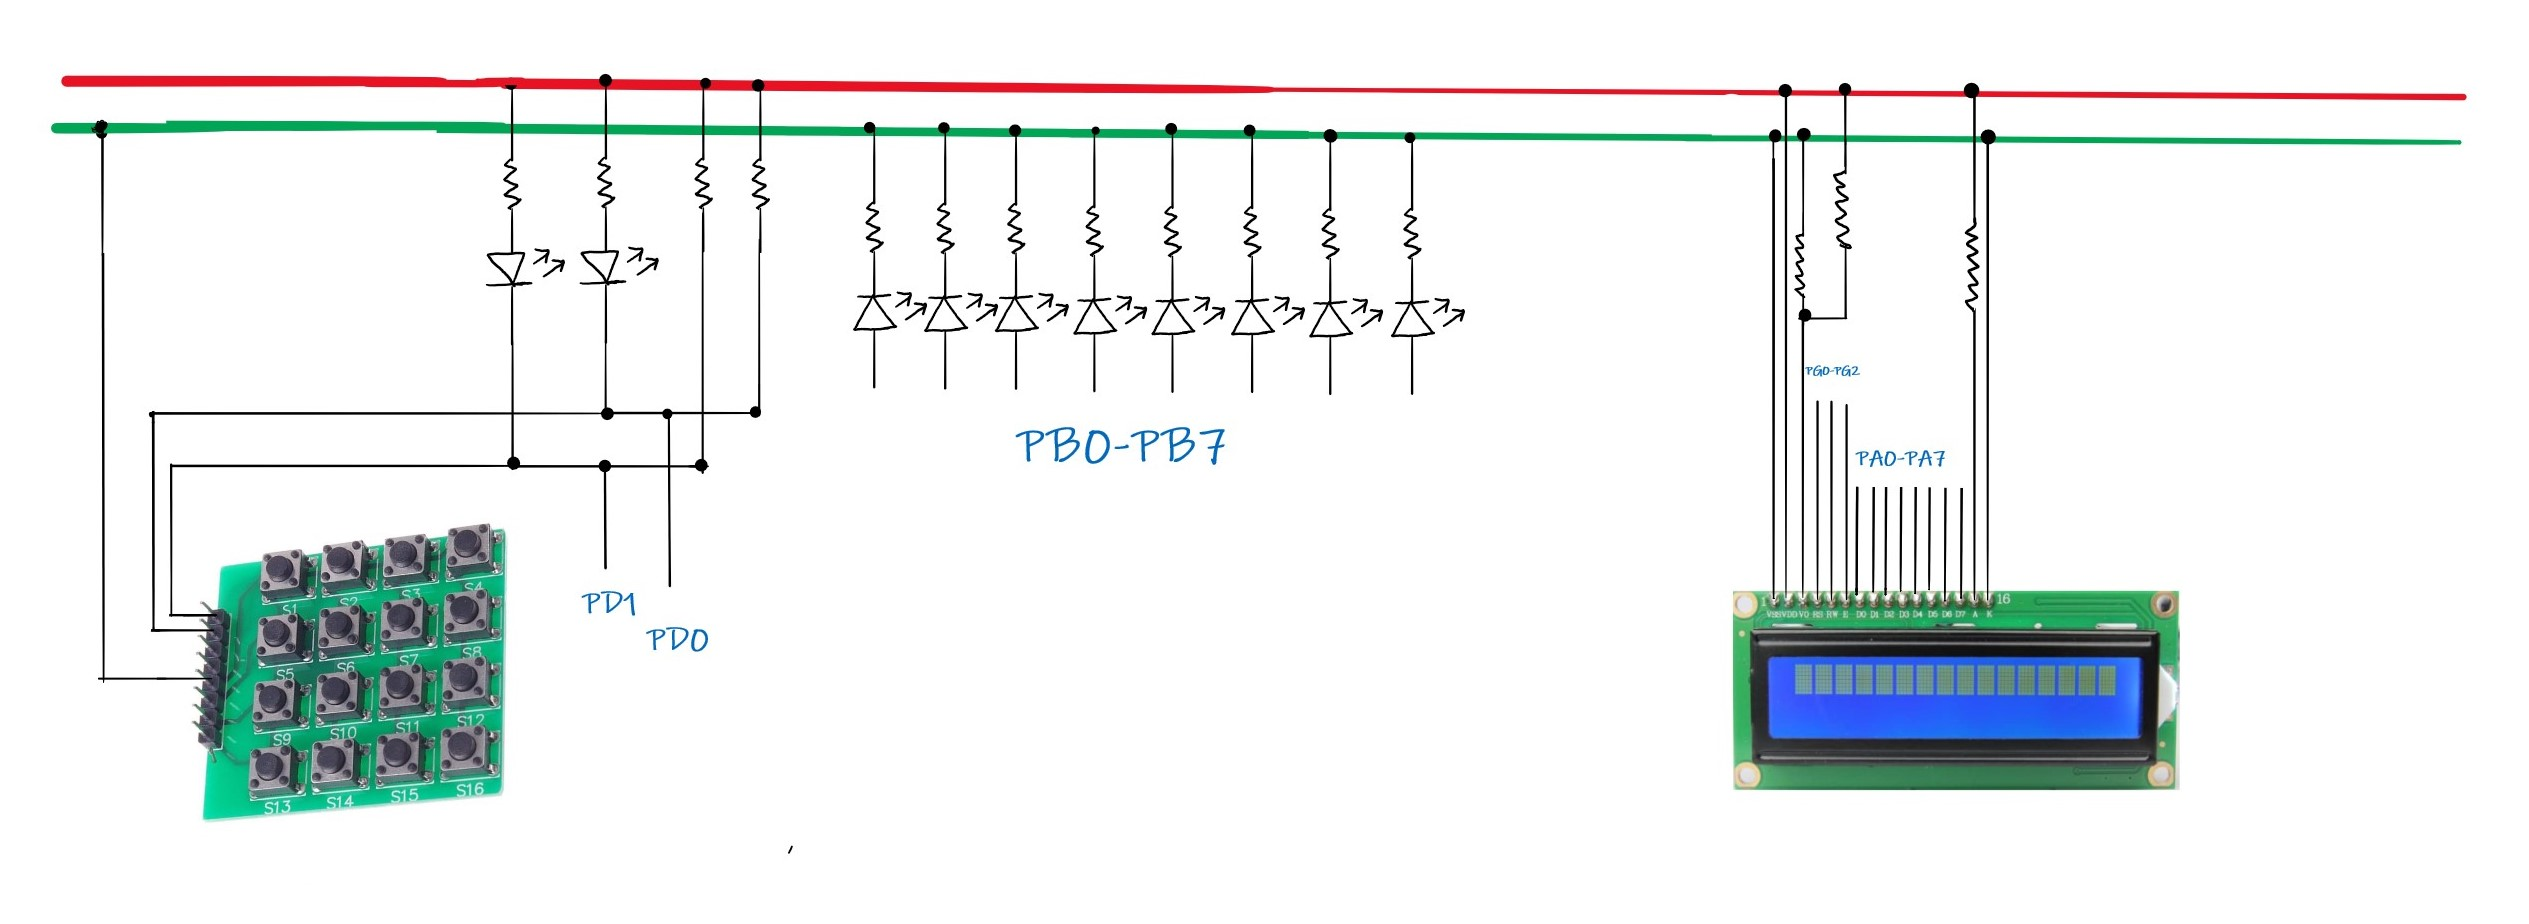
\includegraphics[width=1.1\linewidth,keepaspectratio]{slotschematic.jpg}
}
\caption{Circuit Diagram }
\label{Fig_Circuit_Diagram}
\end{figure}

\begin{figure}[h]
\centering{
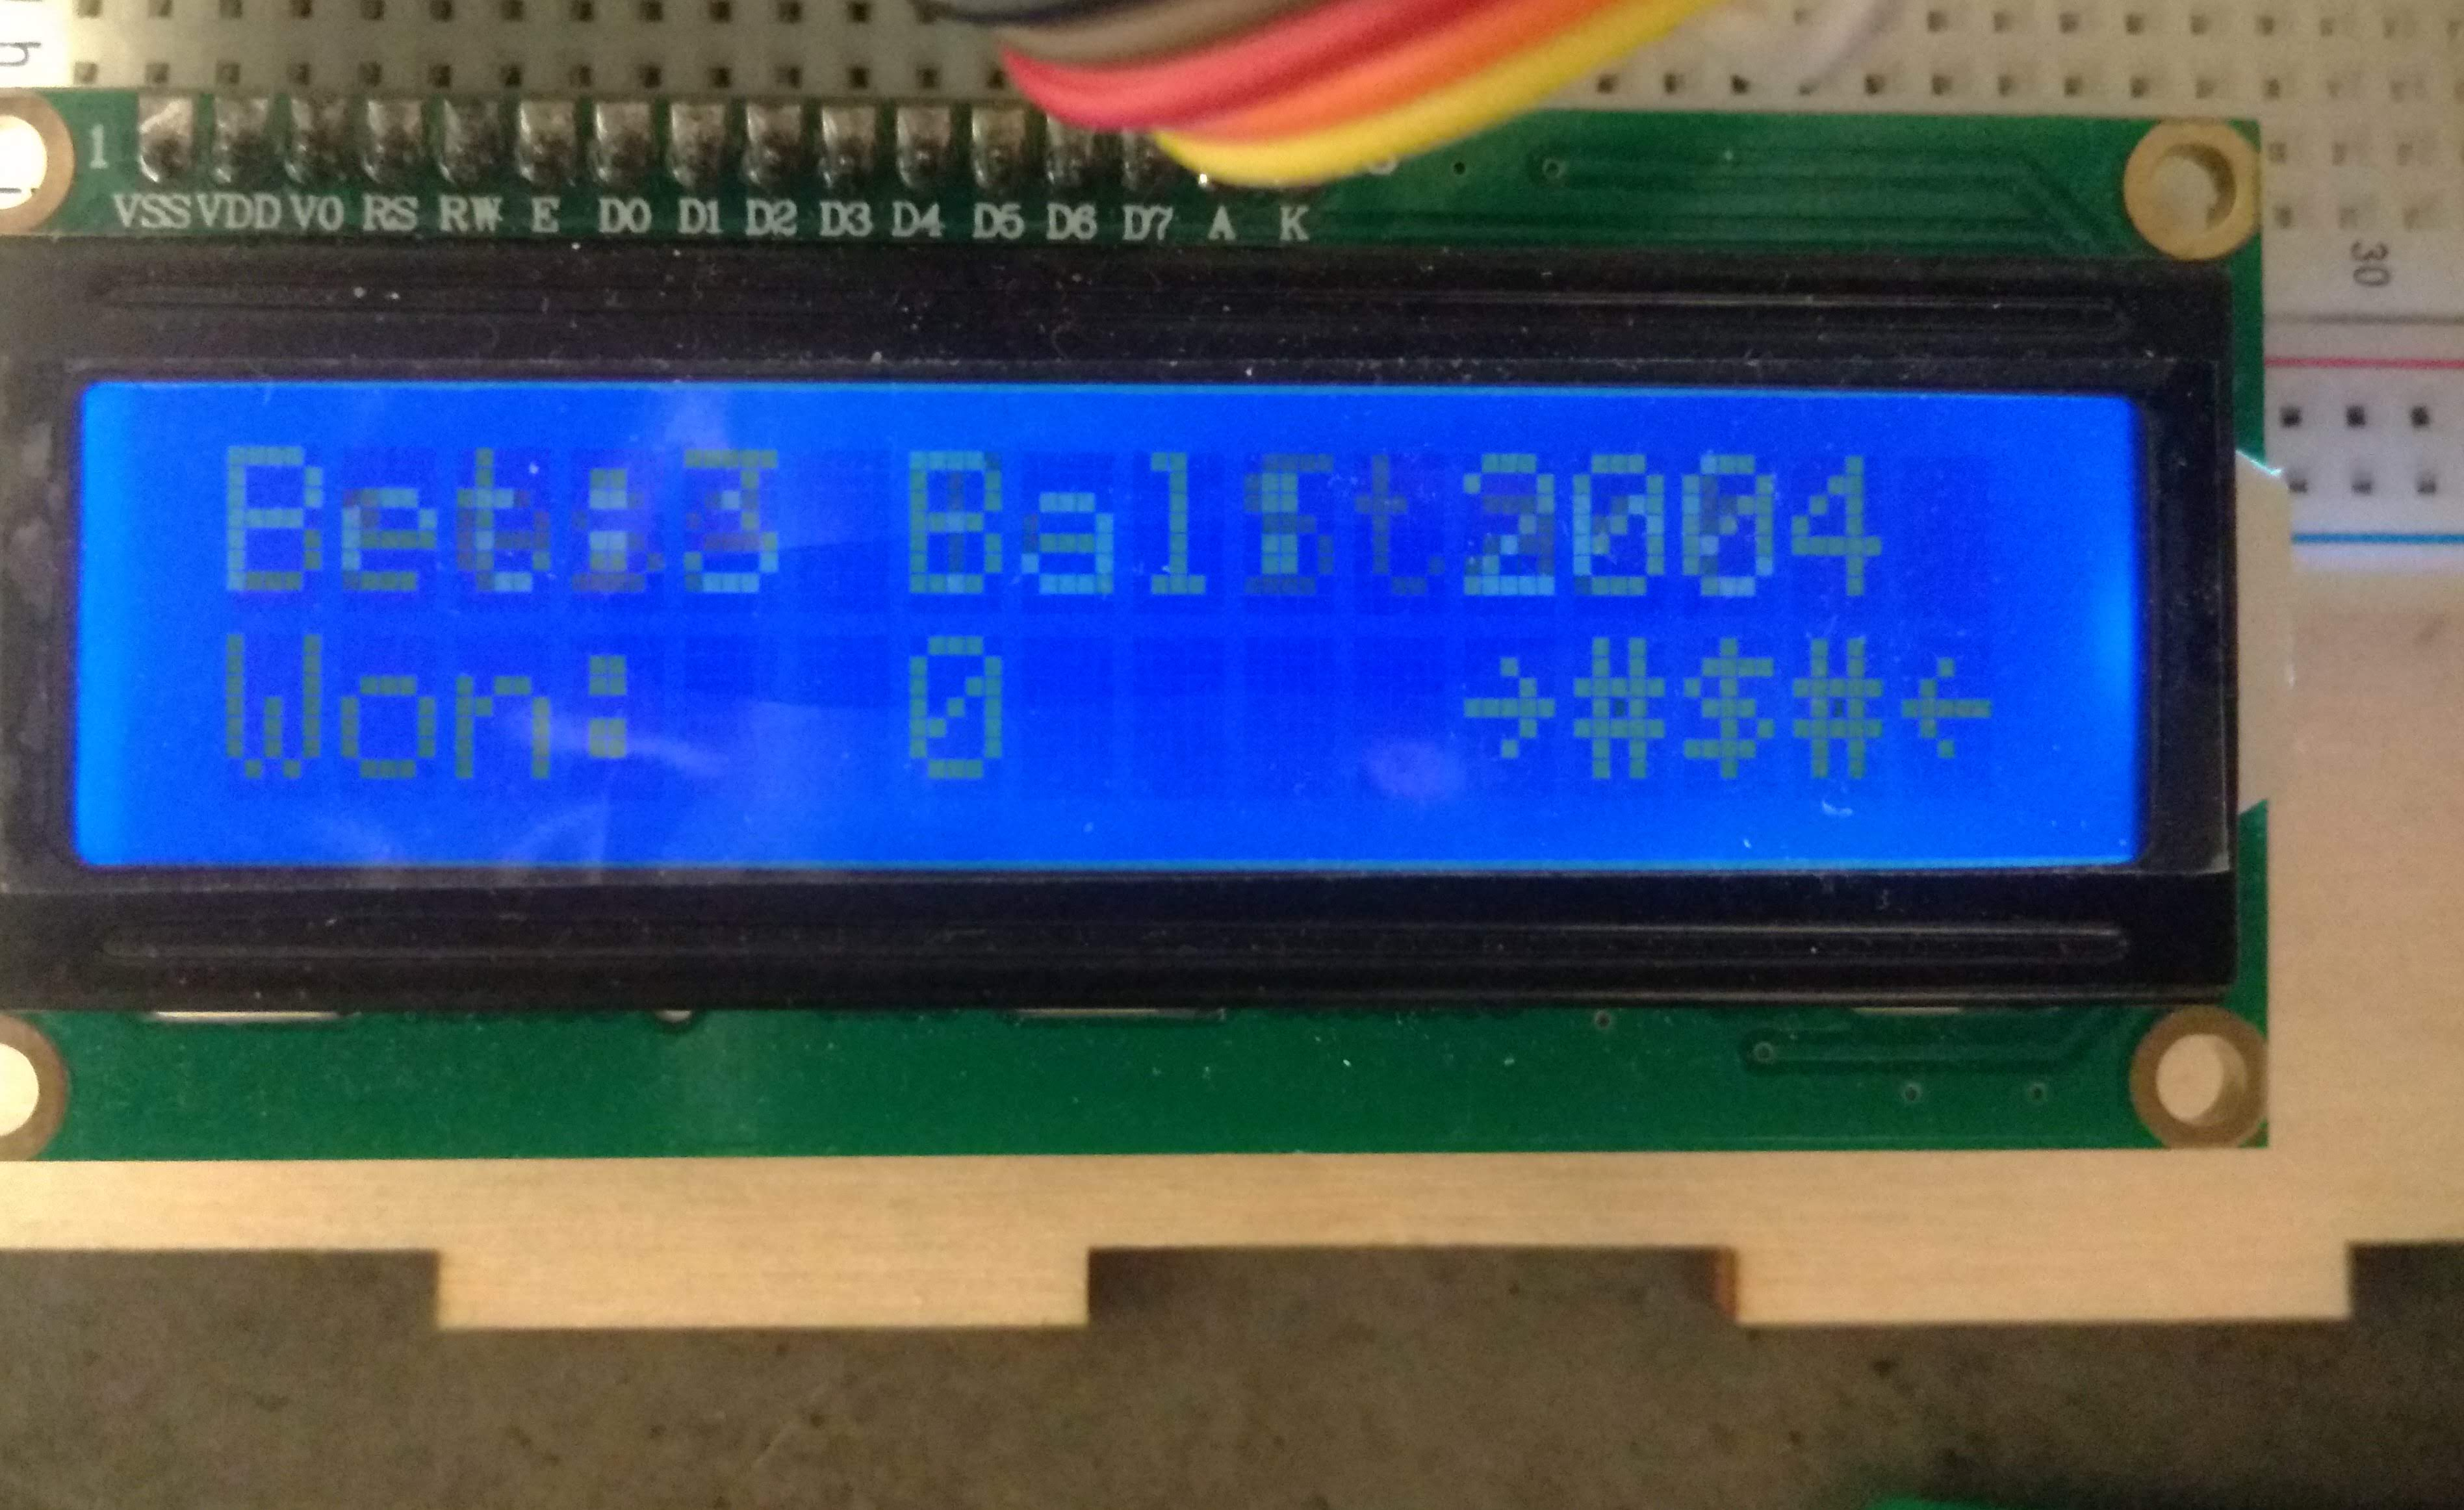
\includegraphics[width=\linewidth,keepaspectratio]{LCD_Slot_Machine.jpg}
}
\caption{LCD Display }
\label{Fig_LCD_Split}
\end{figure}
The life-size slot machine's spin and bet levers are realized by buttons. The life-size screen is realized by LCD. The LCD is divided into four sections:- bet section, balance section, winning amount section and wheel section. Figure \ref{Fig_LCD_Split} shows the division of section on LCD. The lighting effect is realized with 8 leds. The initial balance is set to 2000. Default bet value is 1. The three wheels of slot machine is represented by 3 led characters in the wheel section of LCD. Spin button is given higher priority interrupt then the bet button. Timer 1 is used to check the activity time out. Activity time out is set to 20 seconds.  


\break
Timing requirements for the system are
\begin{itemize}
\item the response on button pressed should reflect on LCD within 1 sec.
\item the wheel spinning should not be so fast that the change of symbols on the screen is not observable.
\item the wheel spinning should not be so slow that player gets enough time to stop by seeing symbol at screen.
\end{itemize}


\large \textbf{ Game Logic:}

\begin{itemize}
\item pressing bet button increases bet
\item pressing spin button toggles the spin functionality 
\item when spin is stopped and the wheels match the reward pattern, the balance is increased with reward
\item when spin is stopped and the wheels don't match the reward pattern, the bet value is deducted from balance
\item player wins the game, if the balance is reached to max value 10,000
\item player loses the game, if the balance becomes zero.
\end{itemize}

\newpage
Symbols used for spinning wheels are \(\$\) (dollar), \(Y\) (Yen), \(\#\) (pound), \(\sum\) (summation) and \(\pi\) (pi). There are three placeholders in LCD for 3 wheels. Each of these values are initialized with random seed when system is reset. The three wheels spin at different rate, 2nd wheel's spin is twice slower than first and 3rd wheel spins trice slower than first. The reward is matched with specific patterns and they are listed below. 

\large \textbf {Reward Patterns:}

\begin{itemize}
\item \normalsize \( \pi\ sym\ sym = bet * 5 \)  [ pi and other two same symbol except \(\pi\) ] 
\item \( \$ \$ \$ = bet * 10 \)  
\item \( Y Y Y = bet * 20  \)
\item \( \# \# \# = bet * 30 \) 
\item \tiny \( \sum \sum \sum\) \normalsize = bet * 50
\item \normalsize \( \pi \pi \pi = bet * 100 \)   
\end{itemize}
 
The probability of reward pattern can be expressed as \( \frac{9}{5!} \).

\newpage
The main loop initializes the values and runs SM\_SpinWheel() function in infinite loop. The flow chart of main loop is shown in figure \ref{Fig_Main_Loop}. SM\_SpinWheel checks for spin is started or stopped. When started, it updates the spinning wheels with delay of 100 ms. When stopped it updates the reward win and balance. When spin is stopped activity timeout timer is started. When spin gets started the timer is stopped. When spin is ON the bet button is disabled. When spin is stopped, the spin button is disabled until the LCD is updated with proper values of win and balance. The function SM\_SpinWheel is listed in listing \ref{lst_sm_spin_wheel}. 

\begin{lstlisting}[numbers=left, breaklines=true,caption={ SM\_SpinWheel Function },label={lst_sm_spin_wheel},language=C]

void SM_SpinWheel()
{
	KP_Enable_Spin();
	int count = 1;
	if (gGameData.smState == SM_USER_WAIT)
	{
		SM_EnableIdleTimer();
		gGameData.smState = SM_IDLE_TIMER_START;
	}
	if(SPIN_OFF == spinReels) return;
	SM_DisableIdleTimer();
	gGameData.smState = SM_SPIN;
    KP_Disable_Bet();
    KP_Disable_Bet_Max();
	SM_LightsOff();
    while(SPIN_ON == spinReels)
    {
	   KP_Enable_Spin(); 	
       gGameData.wheel1Pos = ( gGameData.wheel1Pos + 1 ) %spinWheelValuesLength;
       if (count % 2 == 0) gGameData.wheel2Pos = ( gGameData.wheel2Pos + 1 ) %spinWheelValuesLength;
       if (count % 3 == 0) gGameData.wheel3Pos = ( gGameData.wheel3Pos + 1 ) %spinWheelValuesLength;
	   if (count >= 3)
	   {
		    count = 1;
	   }
	   else
	   {
	   	   count++;
	   }
        SM_UpdateLCDReels();
		SM_SpinningLights();
       _delay_ms(SPIN_DELAY);
    }
	KP_Disable_Spin();
    

    gGameData.winValue = SM_WinValue();
    if (gGameData.winValue == 0 )
    {
        if (gGameData.playerData.Balance >= gGameData.playerData.Bet)
        {
            gGameData.playerData.Balance -= gGameData.playerData.Bet;
        }
        else
        {
            gGameData.playerData.Balance = 0;
        }
        if ( 0 == gGameData.playerData.Balance)
        {
            
            SM_GameOver();
			_delay_ms(DISPLAY_BANNER_DELAY);
			SM_InitGameData();
			LCD_Clear();
        }
    }
    else
    {
		SM_BetWonLights();
        gGameData.playerData.Balance += gGameData.winValue;
        if (gGameData.playerData.Balance >= MAX_WIN_BALANCE)
        {
            gGameData.playerData.Balance = MAX_WIN_BALANCE;
            SM_Winner();
			gGameData.smState = SM_IDLE;
			_delay_ms(DISPLAY_BANNER_DELAY);
			SM_InitGameData();
			LCD_Clear();	
        } 

    }
    SM_UpdateLCD();
	KP_Enable_Spin();
    KP_Enable_Bet();
    KP_Enable_Bet_Max();
	gGameData.smState = SM_USER_WAIT;
	SM_UserWaitLights();
}
\end{lstlisting}
 
\begin{figure}[h]
\centering{
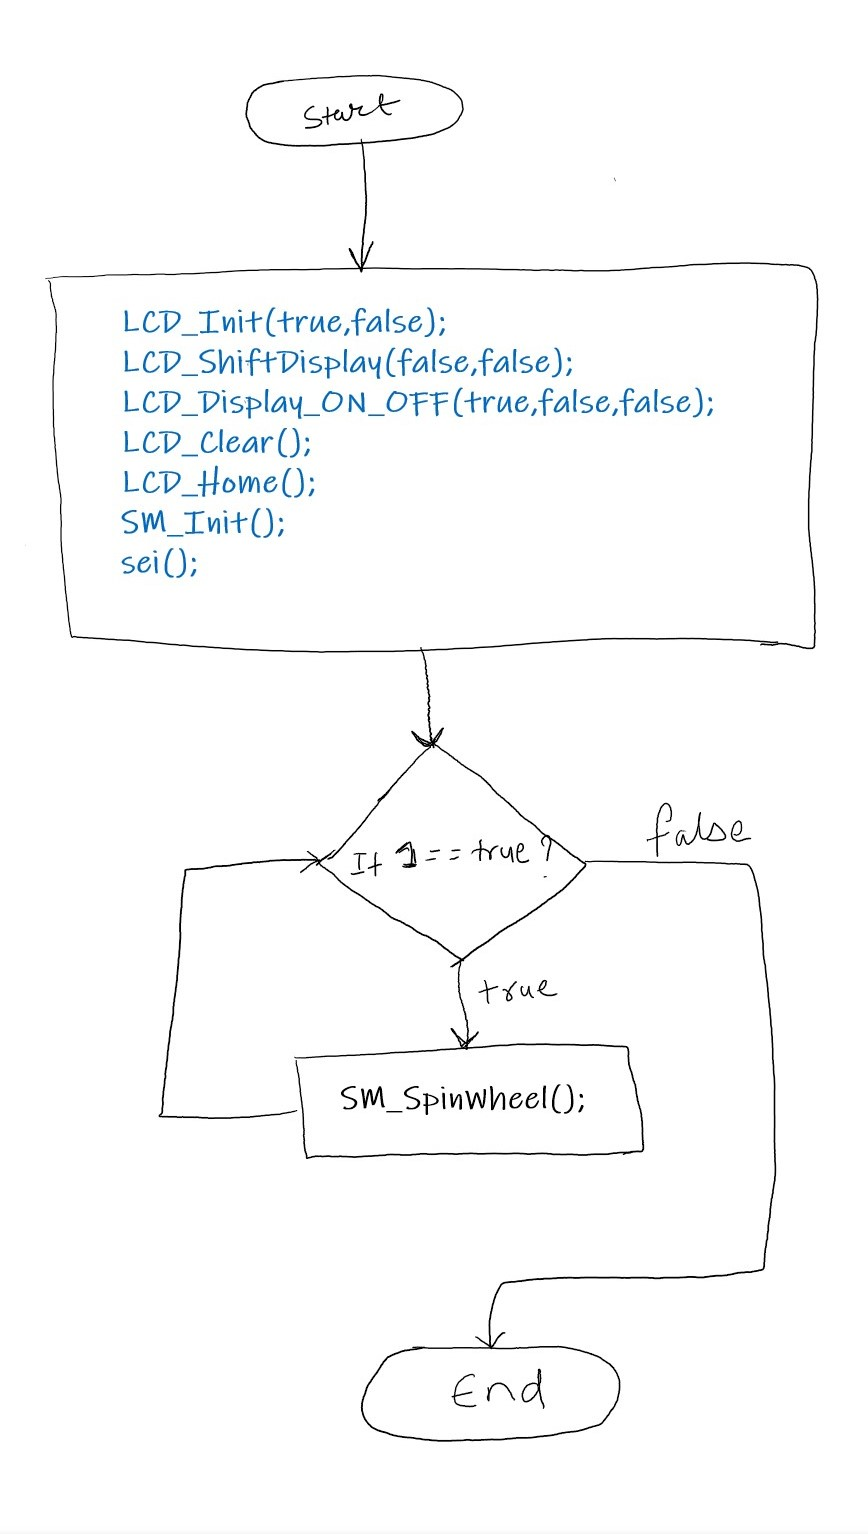
\includegraphics[height=0.7\textheight,width=\linewidth,keepaspectratio=true]{MainFlowchart.jpg}
}
\caption{Main Loop flow chart }
\label{Fig_Main_Loop}
\end{figure}


\clearpage
INT1 and INT0 are used for external interrupts. The interrupt sense is set to falling-edge triggered. The snippet of the code is shown in listing \ref{lst_ext_interrupt}.
\begin{lstlisting}[numbers=left,breaklines=true,caption={External interrupts initialization },label={lst_ext_interrupt},language=C]
	EICRA = 0b00001111;		// INT 3,2 not used, Interrupt Sense (INT1, INT0) falling-edge triggered
	EICRB = 0b00000000;		// INT7 ... 4 not used
	
	EIMSK = 0b00000011;		// Enable INT1, INT0
	EIFR = 0b00000011;
    KEYPAD_DD = INPUT_MODE;
\end{lstlisting}
The spin button is mapped to external interrupt 0.  The flow chart of ISR0 is shown in figure \ref{Fig_ISR0_Loop}. In ISR, spin value is toggled, lights patterns are set, interrupt 0 is disabled and interrupt flags are cleared off, if state is not STATE\_IDLE. In STATE\_IDLE, the state is changed to STATE\_USER\_WAIT, LCD is updated with game visuals and flags are cleared off. 


\begin{figure}[h]
\centering{
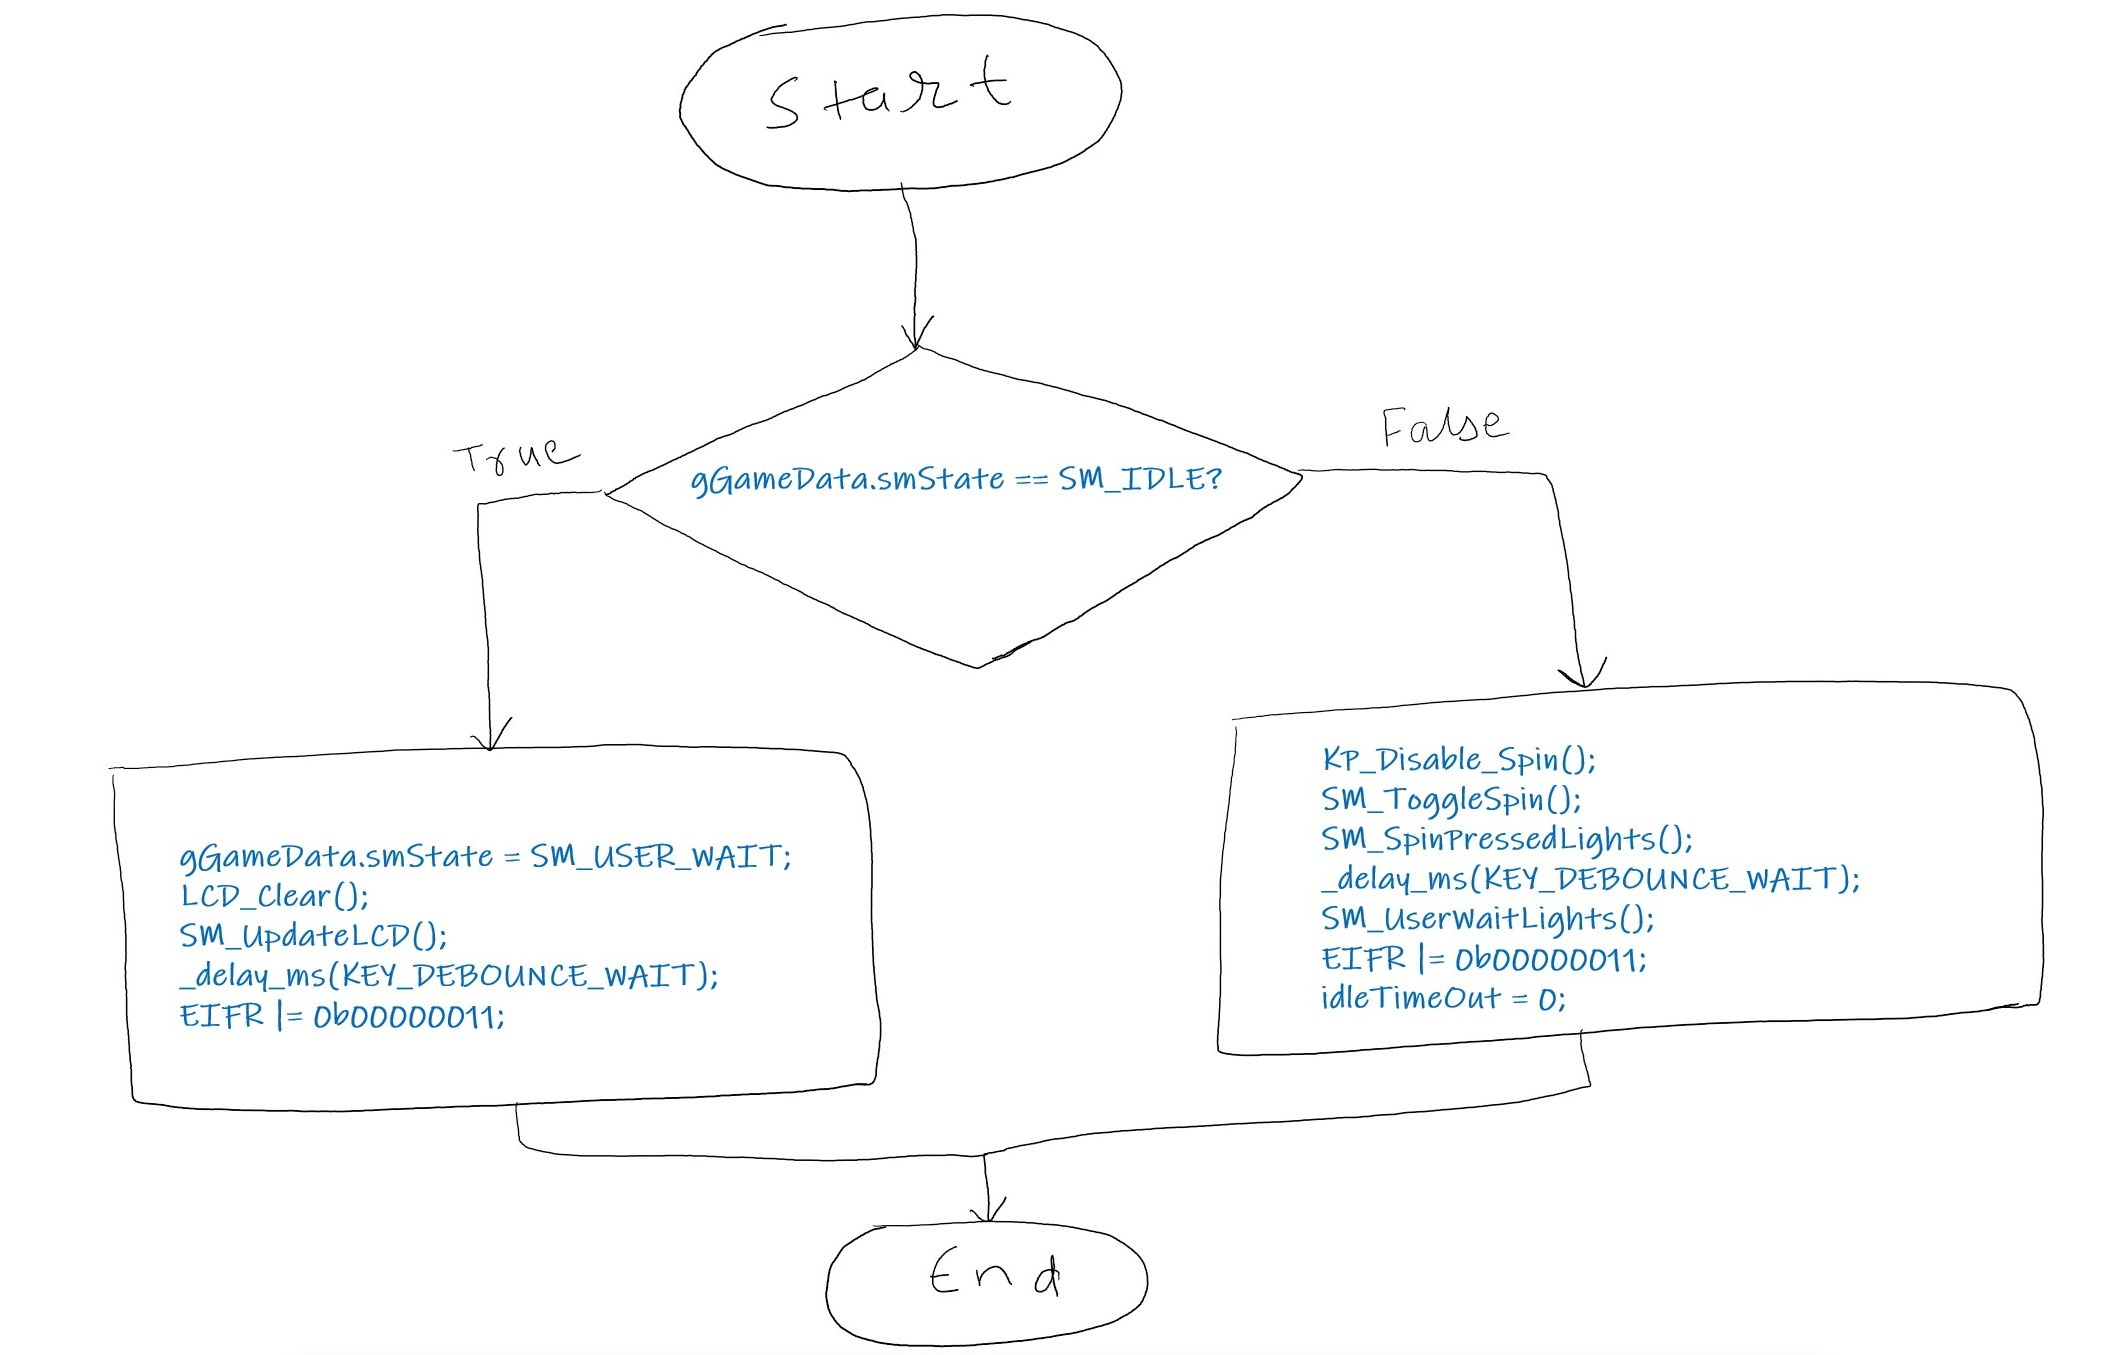
\includegraphics[height=\textheight,width=\linewidth,keepaspectratio]{ISR0Loop.jpg}
}
\caption{ISR0 / spin button flow chart }
\label{Fig_ISR0_Loop}
\end{figure}


\clearpage

 The bet button is mapped to external interrupt 1. The flow chart of ISR1 is shown in figure \ref{Fig_ISR1_Loop}. In ISR1 when state is not STATE\_IDLE, the external interrupts are disabled, bet value is increased, bet value is updated on screen, light patterns are set, interrupt flags are cleared off and then external interrupts are enabled. In STATE\_IDLE, the state is changed to STATE\_USER\_WAIT, LCD is updated with game visuals and flags are cleared off.    


\begin{figure}[h]
\centering{
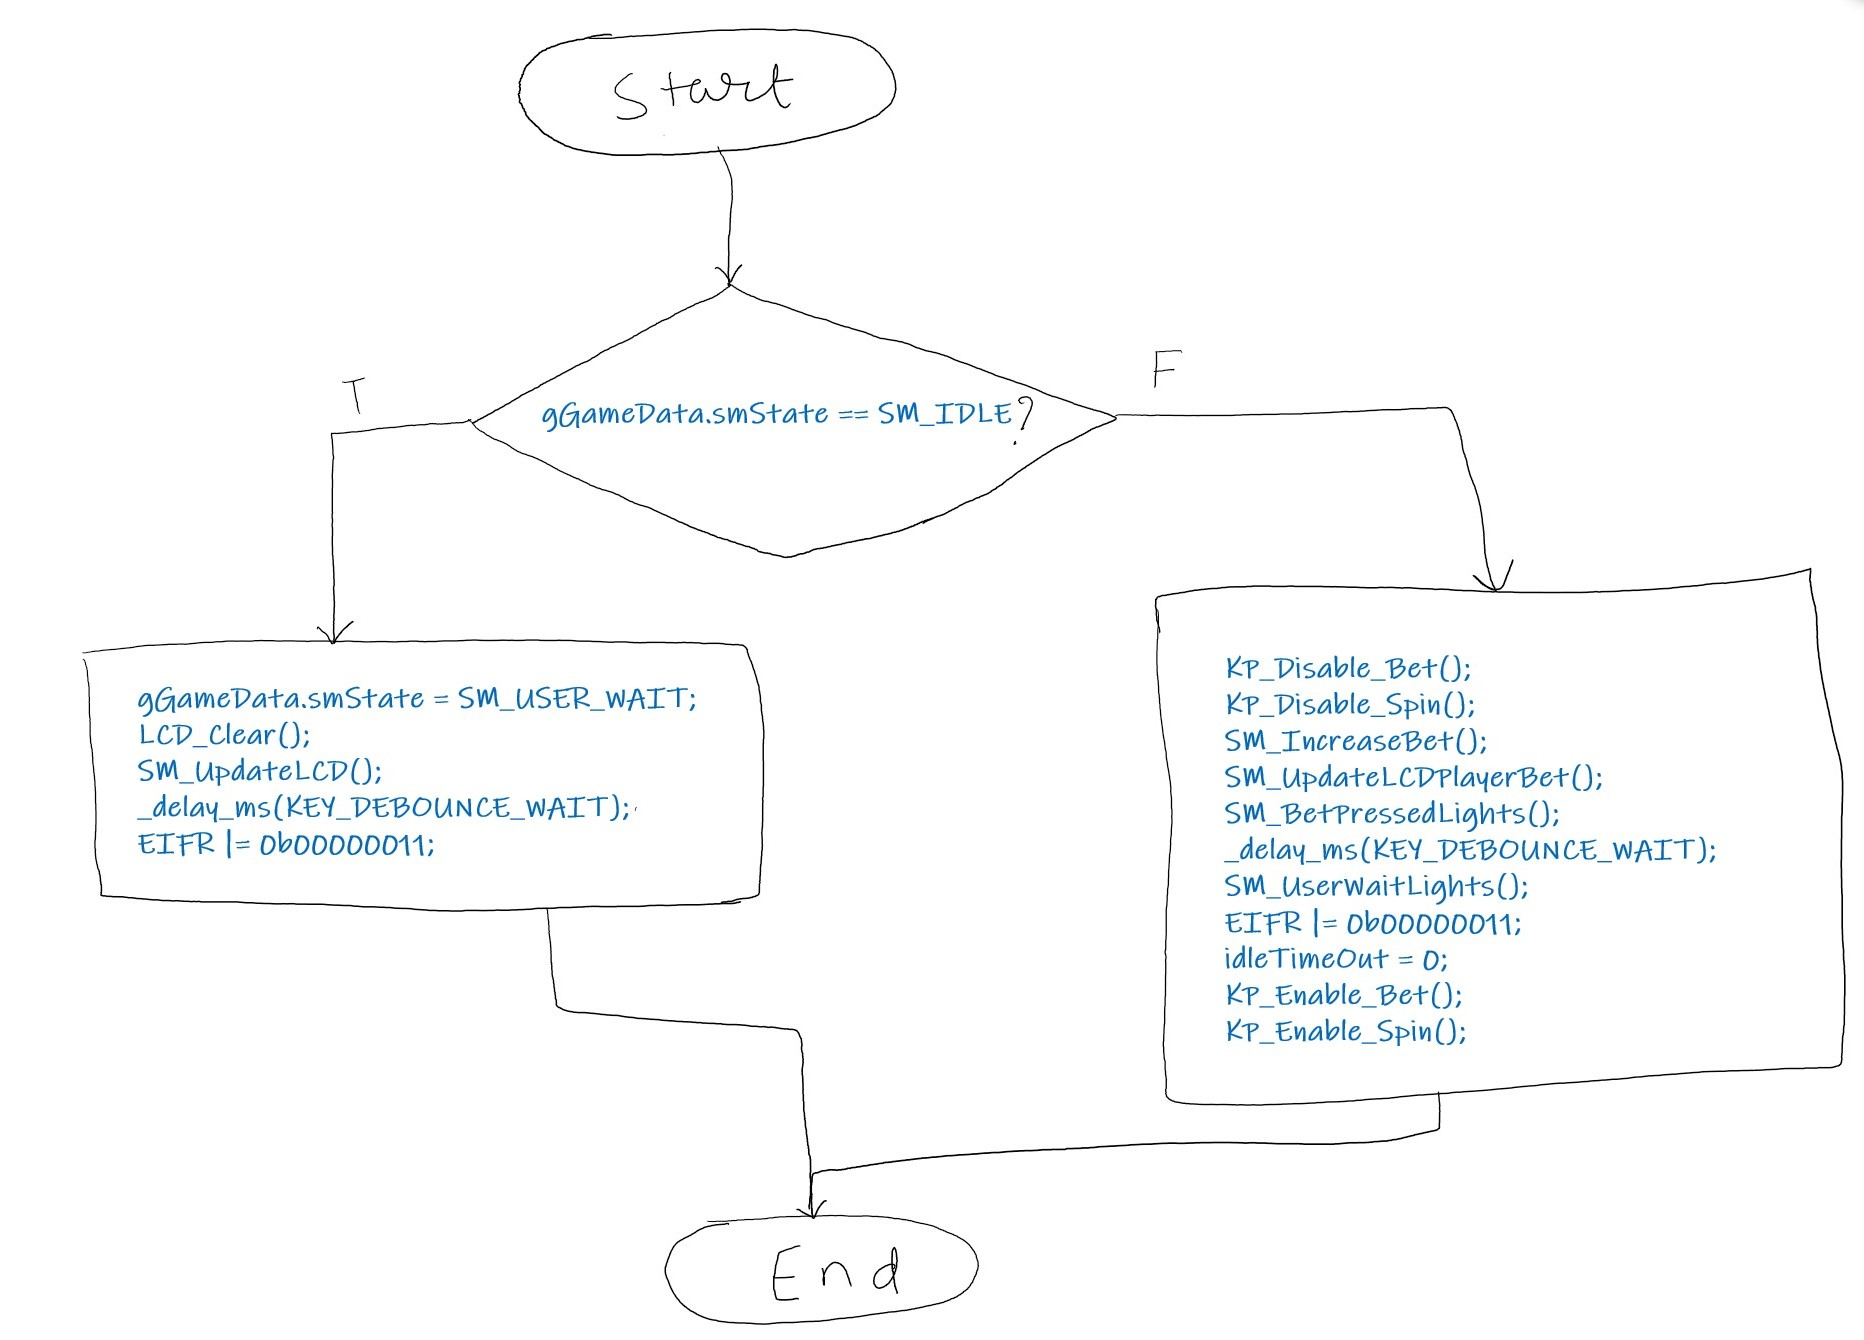
\includegraphics[height=\textheight,width=\linewidth,keepaspectratio]{ISR1Loop.jpg}
}
\caption{ISR1 / bet button flow chart }
\label{Fig_ISR1_Loop}
\end{figure}

Timer 1 is used for checking the inactivity of player. Timer initialization is done in function SM\_InitialiseIdleTimer(). The code snippet for timer interrupt on every 1 sec is listed in \ref{lst_timer1}. If the inactivity is for more than 20 sec, the screen throws "Press to Play" to message. The flow chart for ISR for Timer is shown in figure \ref{Fig_ISR_Timer0}. 

\begin{lstlisting}[numbers=left, breaklines=true, caption={Timer 1 initialization },label={lst_timer1},language=C]
	TCCR1A = 0b00000000;    // Normal port operation (OC1A, OC1B, OC1C), Clear Timer on 'Compare Match' (CTC) waveform mode)
	TCCR1B = 0b00001000;    // CTC waveform mode, initially stopped (no clock)
	TCCR1C = 0b00000000;

	// clock = 1 MHz , prescaler = 1024,
    // to achieve  1 second interval:
	// Need to count 1 million clock cycles (but already divided by 1024)
	// So actually need to count to (1000000 / 1024 =) 976 decimal, = 3D0 Hex
	OPER_16_BIT_START
	OCR1AH = 0x03; // Output Compare Registers (16 bit) OCR1BH and OCR1BL
	OCR1AL = 0xD0;
	OPER_16_BIT_END

	
	TIMSK1 = 0b00000010;    // bit 1 OCIE1A         Use 'Output Compare A Match' Interrupt, i.e. generate an interrupt
	// when the timer reaches the set value (in the OCR1A register)
\end{lstlisting}
\begin{figure}[h]
\centering{
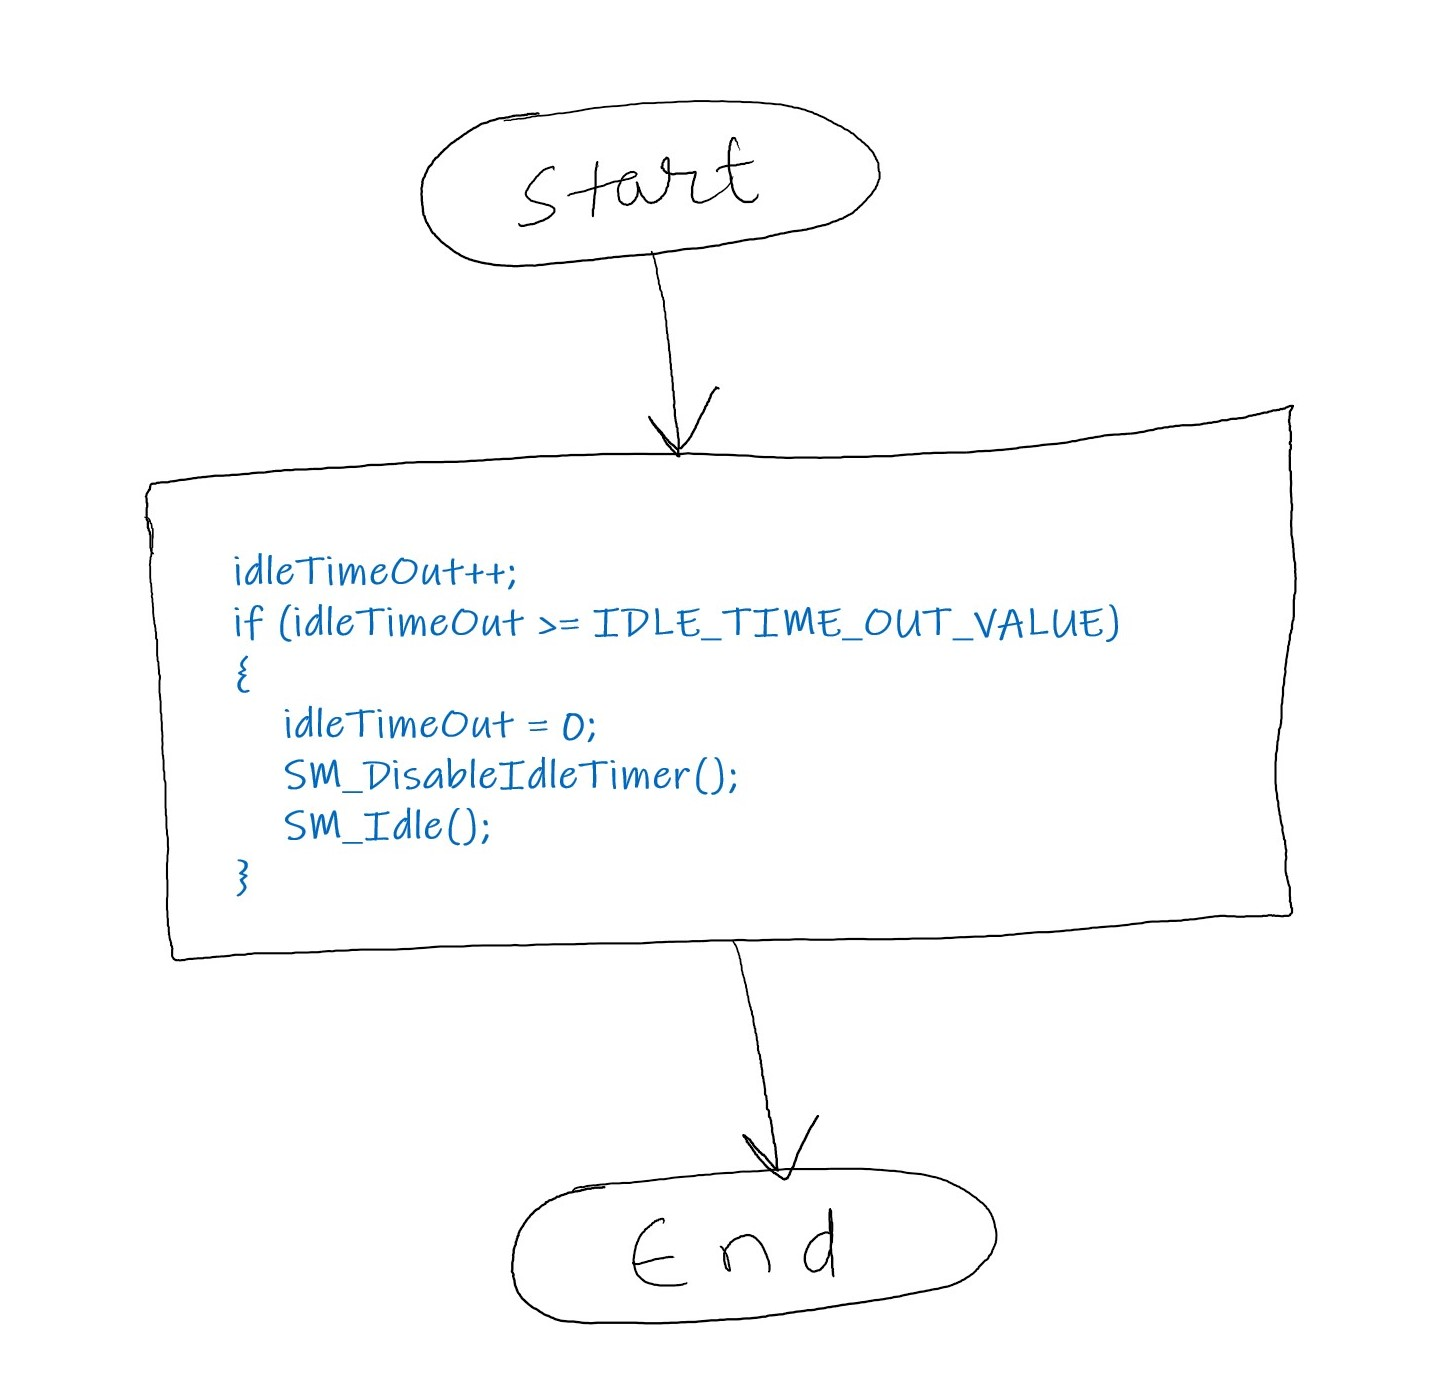
\includegraphics[height=\textheight,width=\linewidth,keepaspectratio]{ISR_Timer0.jpg}
}
\caption{ISR Timer0 / Activity timeout flow chart }
\label{Fig_ISR_Timer0}
\end{figure}

\clearpage
\newpage
There are 5 states in this design, and they are SM\_INIT, SM\_USER\_WAIT, SM\_IDLE\_TIMER\_START, SM\_SPIN, SM\_IDLE. The state transition is shown in figure \ref{Fig_State_Diagram}. 

\begin{figure}[h]
\centering{
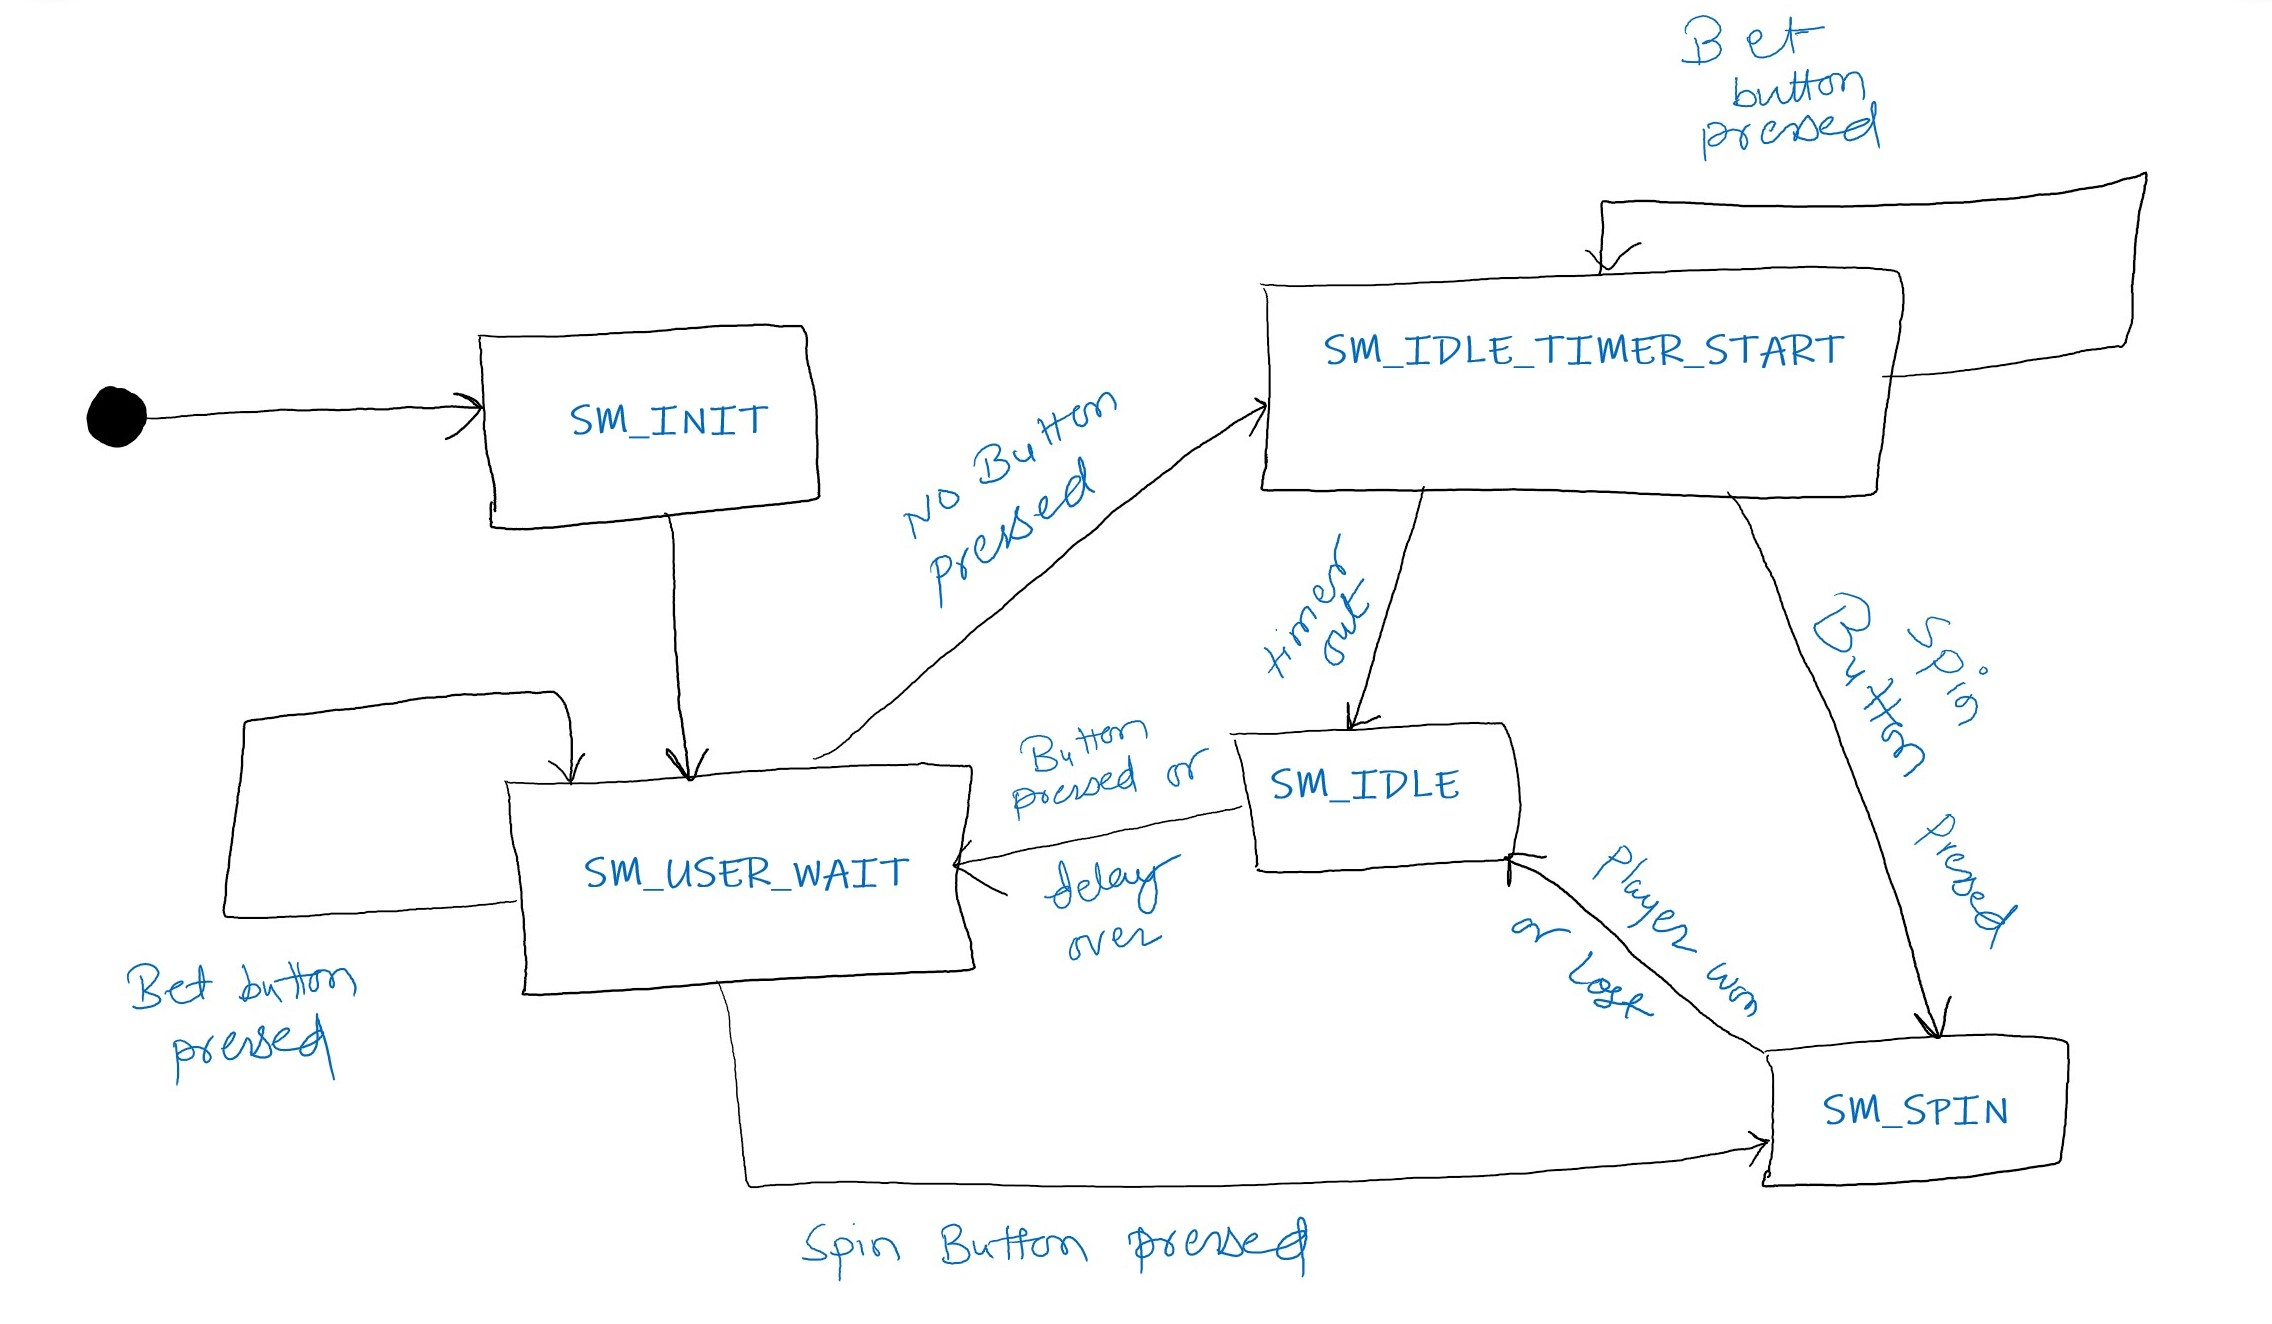
\includegraphics[height=0.7\textheight,width=\linewidth,keepaspectratio]{stateDiagram.jpg}
}
\caption{State Diagram }
\label{Fig_State_Diagram}
\end{figure}

\newpage
\section{Timing Diagram}
Three timing diagram shows when three different interrupts are triggered.   

\begin{figure}[h]
\centering{
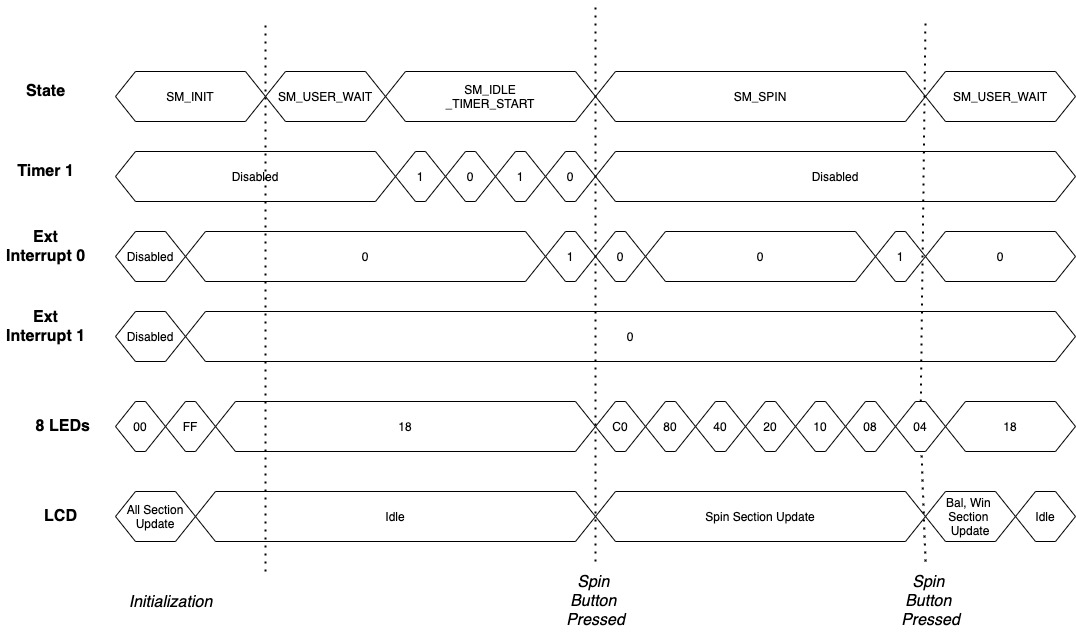
\includegraphics[height=0.7\textheight,width=\linewidth,keepaspectratio]{Timing_slotMachine-Spin_timing.jpg}
}
\caption{Timing diagram when spin button is pressed }
\label{Fig_Spin_Timing}
\end{figure}

\begin{figure}[h]
\centering{
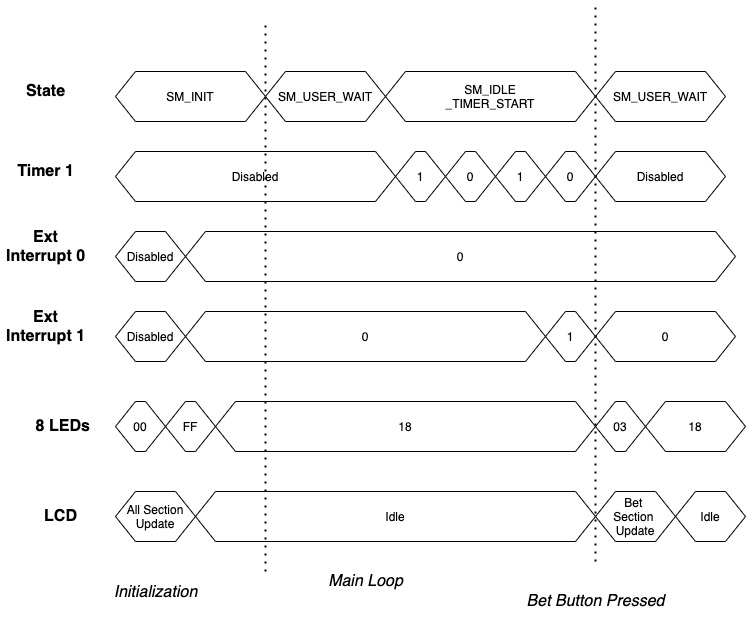
\includegraphics[height=0.7\textheight,width=\linewidth,keepaspectratio]{Timing_slotMachine-Bet_Timing.jpg}
}
\caption{Timing diagram when bet button is pressed }
\label{Fig_Bet_Timing}
\end{figure}

\begin{figure}[h]
\centering{
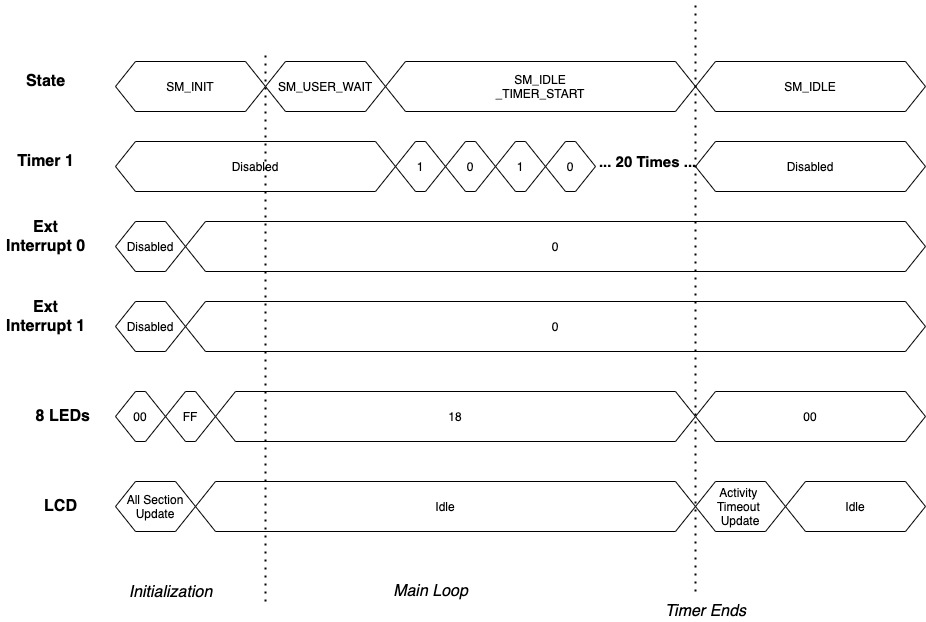
\includegraphics[height=0.7\textheight,width=\linewidth,keepaspectratio]{Timing_slotMachine-Timer1_expires.jpg}
}
\caption{Timing diagram when activity timeout timer expires }
\label{Fig_Timer_Timing}
\end{figure}

\chapter {Testing}
Black box and white box testings were done for the project. The list of test cases is listed below in tabular form.

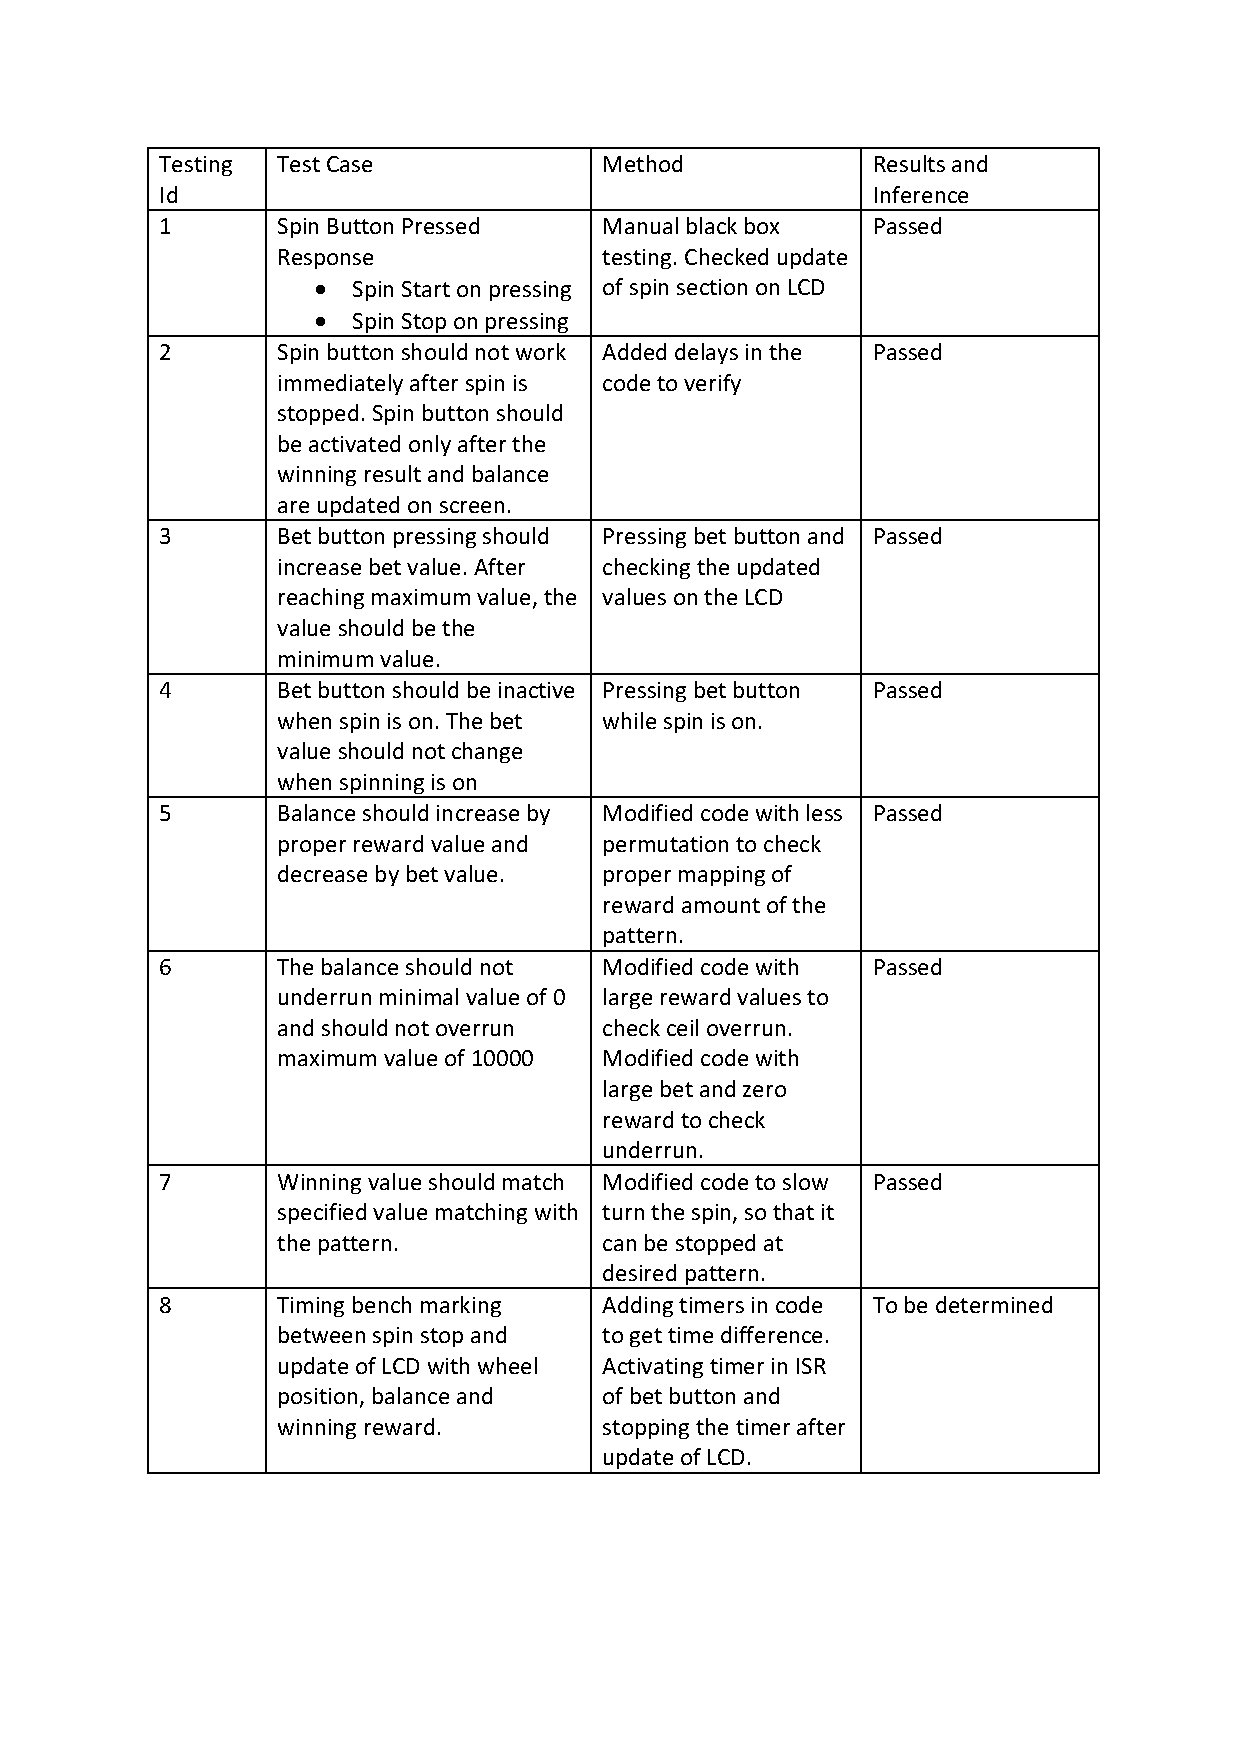
\includepdf[pages=-]{Testing_Matrix.pdf}

The Worst Case Execution Time (WCET) can be considered for the time of response when the spin is stopped, and the values get updated. Considering 1Mz clock speed, 37 \(\mu\)s write and command time for LCD, WCET can be calculated from code walk through. In function SM\_SpinWheel() in file SlotMachine.c, a while loop runs when spin is on, i.e. \textbf{while(SPIN\_ON == spinReels)}. It is considered the main routine is exactly at this point when ISR routine for spin button is pressed. The longest code path till the LCD update occurs give the WCET. No reward pattern is considered for the longest code traversal. The calculated WCET rounds off to 104 ms.


\chapter {Source Listing}

 The source code files developed in this project are:
\begin{itemize}
\item Config.h \\*
    Configuration of the ports and abstract macros defined here.
\item KeyPad.h \\*
    Buttons related functions are declared here.
\item LcdLibrary.h \\*
    LCD related functions are declared, and related macros are defined here.
    
\item SlotMachine.h \\*
    Game related data structure and variables are declared here.
\item KeyPad.c \\*
    Functions of KeyPad.h are defined here.
\item LcdLibrary.c \\*
    Functions of LcdLibrary.h are defined here.
\item SlotMachine.c \\*
    Functions of SlotMachine.h are defined here. The main logic implementation and trigger are written here.
\item main.c \\*
    Main and ISR routines are defined here.
    
\end{itemize}

The source code is also available at \href{https://github.com/simplybiplav/SlotMachine}{github}.


\section{Config.h}
\begin{small}
\lstinputlisting[language=c,breaklines=true,numbers=left,tabsize=4]{../SlotMachineAtmelProject/SlotMachineAtmelProject/Config.h}
\end{small}

\newpage
\section{LcdLibrary.h}
\begin{small}
\lstinputlisting[language=c,breaklines=true,numbers=left,tabsize=4]{../SlotMachineAtmelProject/SlotMachineAtmelProject/LcdLibrary.h}
\end{small}

\newpage
\section{KeyPad.h}
\begin{small}
\lstinputlisting[language=c,breaklines=true,numbers=left,tabsize=4]{../SlotMachineAtmelProject/SlotMachineAtmelProject/KeyPad.h}
\end{small}

\newpage
\section{SlotMachine.h}
\begin{small}
\lstinputlisting[language=c,breaklines=true,numbers=left,tabsize=4]{../SlotMachineAtmelProject/SlotMachineAtmelProject/SlotMachine.h}
\end{small}


\newpage
\section{LcdLibrary.c}
\begin{small}
\lstinputlisting[language=c,breaklines=true,numbers=left,tabsize=4]{../SlotMachineAtmelProject/SlotMachineAtmelProject/LcdLibrary.c}
\end{small}


\newpage
\section{KeyPad.c}
\begin{small}
\lstinputlisting[language=c,breaklines=true,numbers=left,tabsize=4]{../SlotMachineAtmelProject/SlotMachineAtmelProject/KeyPad.h}
\end{small}


\newpage
\section{SlotMachine.c}
\begin{small}
\lstinputlisting[language=c,breaklines=true,numbers=left,tabsize=4]{../SlotMachineAtmelProject/SlotMachineAtmelProject/SlotMachine.c}
\end{small}


\newpage
\section{Main.c}
\begin{small}
\lstinputlisting[language=c,breaklines=true,numbers=left,tabsize=4]{../SlotMachineAtmelProject/SlotMachineAtmelProject/Main.c}
\end{small}




\chapter {Critical evaluation and Conclusion}
All the major aspects and functionalities of the project are developed.The developed project works almost perfectly as intended. The developed system is shown in the figure \ref{Fig_Slot_Machine_Realised}. There is one unfinished work of maximum bet. A button which can set the bet value to maximum, instead of hitting bet button multiples times to reach the max value. The c functions for this is in place but are left unimplemented. The unimplemented code doesn't have any observable major impact on any such functionalities. The button bounce could be addressed by adding extra capacitive circuit for the buttons. The bench marking of time between the spin stop and LCD update hasn't been achieved. There is enough room to add further functionalities to it. One good feature would be to provide interface to configure desired symbols and desired patterns for reward.   

\begin{figure}[h]
\centering{
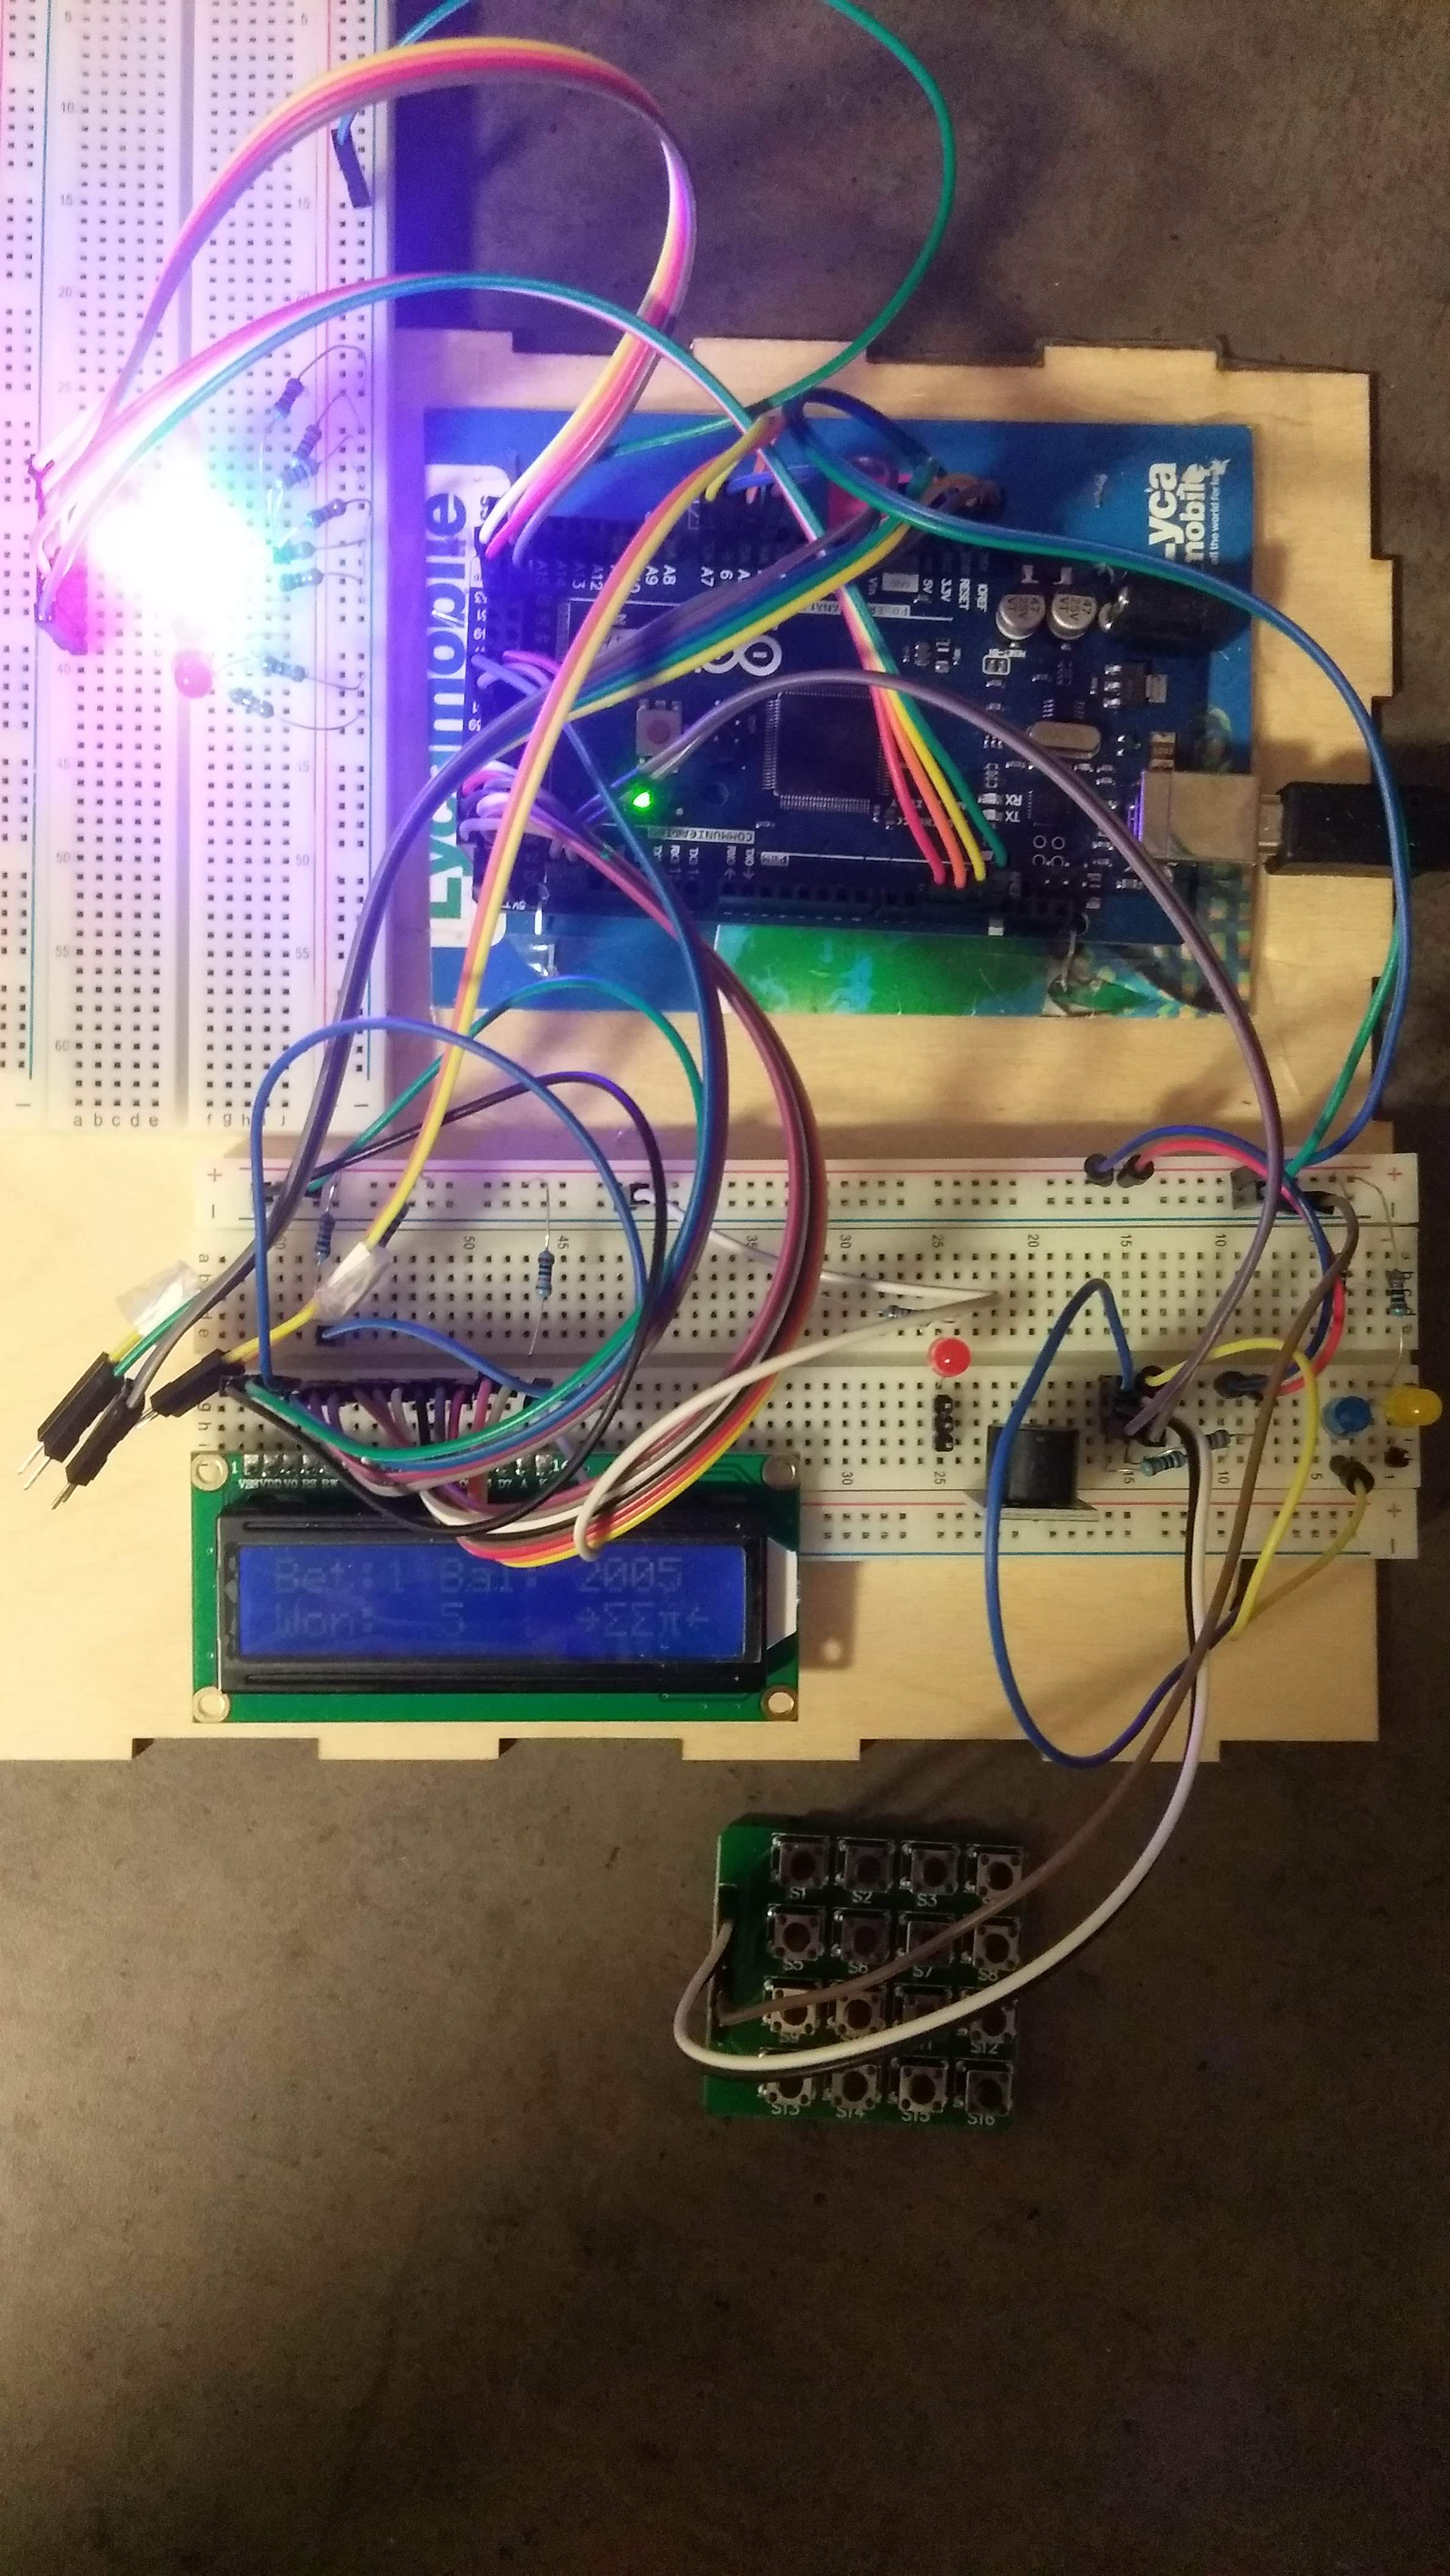
\includegraphics[height=0.5\textheight,keepaspectratio=true]{Slot_Machine.jpg}
}
\caption{Developed Slot Machine}
\label{Fig_Slot_Machine_Realised}
\end{figure}
\end{document}
